\documentclass[11pt,a4paper]{article}

\usepackage[T1]{fontenc}
\usepackage[utf8]{inputenc}
\usepackage[spanish,es-noquoting,es-tabla]{babel}
\usepackage{amsmath,amssymb,amsthm}
\usepackage{mathtools}
\usepackage{csquotes}
\usepackage{array}
\usepackage{booktabs}
\usepackage{graphicx}
\usepackage{caption}
\usepackage{enumitem}
\usepackage[margin=2.4cm]{geometry}
\usepackage{microtype}
\usepackage{xcolor}
\setlength{\emergencystretch}{3em}
\usepackage[colorlinks=true,linkcolor=blue!55!black,citecolor=blue!55!black,
            urlcolor=blue!55!black]{hyperref}

\graphicspath{{figs_crb_ellipses/}{../plots/}}

\newcommand{\vect}[1]{\boldsymbol{#1}}
\newcommand{\matr}[1]{\mathbf{#1}}
\newcommand{\code}[1]{\texttt{#1}}
\newcommand{\dd}{\mathrm{d}}
\DeclareMathOperator{\Cov}{Cov}
\DeclareMathOperator*{\E}{\mathbb{E}}
\DeclareMathOperator{\diag}{diag}
\DeclareMathOperator{\tr}{tr}

\theoremstyle{definition}
\newtheorem{obs}{Observación}
\newtheorem{salvedad}{Salvedad}

\theoremstyle{plain}
\newtheorem{prop}{Proposición}

\title{\textbf{De la tasa esperada a las elipses}\\[2mm]
\large Qu\'e estima la CRB, c\'omo se construye la covarianza\\
y por qu\'e las burbujas tienen esa forma}
\author{Repositorio \code{crb}}
\date{4 de septiembre de 2026}

\begin{document}
\shorthandoff{"}
\maketitle

\begin{abstract}
Este texto cubre \textbf{solo} la mitad estad\'istica del \emph{pipeline}: a
partir del momento en que el simulador ya ha producido la tasa esperada de
fotones $g(\vect\psi)$. No se rederiva la radiometr\'ia ni el rasterizado.
La pregunta que queda es: si un SPAD observara esa tasa con ruido de Poisson,
\textbf{cuánto podríamos saber de la pose} $\vect\psi=(\rho,\varphi)$.
La respuesta no se obtiene simulando estimadores: se obtiene de la matriz de
informaci\'on de Fisher y de su inversa, la cota de Cram\'er--Rao (CRB), que
es una covarianza. De esa covarianza se lee $\sigma_\rho$, $\sigma_\varphi$,
la correlaci\'on, y se dibuja una elipse de radio $k$ en el plano de
par\'ametros. Cada f\'ormula se justifica y se ata al c\'odigo de
\code{crb\_polar\_functions.py}.
\end{abstract}

\tableofcontents
\vspace{0.6em}
\hrule
\vspace{0.8em}

%=======================================================================
\section{Qu\'e problema se resuelve (y qu\'e no)}
\label{sec:problema}

Tenemos un modelo $g(\vect\psi)$: un cubo
$(\text{p\'ixel},\,\text{\emph{bin}})$ de tasas esperadas de fotones, funci\'on
de la pose de la faceta. Lo que \emph{no} tenemos ---y el CRB no necesita---
es una medici\'on ruidosa concreta. El objeto que se calcula es una
\textbf{cota} sobre cualquier estimador razonable de esa pose.

El vector de par\'ametros en el \emph{baseline} actual es
%
\begin{equation}
\label{eq:psi}
\vect\psi = \begin{pmatrix}\rho\\ \varphi\end{pmatrix}
\in \mathbb R^{2}_{>0}\times(0,\pi).
\end{equation}
%
$\rho$ es la distancia al origen en el suelo y $\varphi$ el azimut. El ancho
de la faceta $w$ es un dato de escena, no se estima. La altura no entra:
el simulador de producci\'on no la expone como entrada, as\'i que no existe
$\partial g/\partial h$ y la Fisher es $2\times 2$.

Un \textbf{estimador} ser\'ia una funci\'on $\hat{\vect\psi}(\vect x)$ que, dada
una realizaci\'on ruidosa $\vect x$ del transitorio, devolviera un par
$(\hat\rho,\hat\varphi)$. El de m\'axima verosimilitud, por ejemplo, maximiza
$\ell(\vect\psi;\vect x)$ de la secci\'on~\ref{sec:verosimilitud}. \textbf{Ese
paso no se ejecuta.} No hay bucle de optimizaci\'on, no hay semilla, no hay
promedio Monte Carlo. Lo que se calcula es: si existiera un estimador
insesgado, su covarianza no podr\'ia ser mejor que $\matr I(\vect\psi)^{-1}$.
Dibujar esa matriz como elipse es dibujar \textbf{el mejor error t\'ipico
posible} bajo el modelo, no el error de un algoritmo concreto.

\begin{obs}[El CRB no consume datos]
El \emph{pipeline} llama al \emph{forward} con \code{add\_noise=False}
(\code{force\_no\_noise=True} en \code{compute\_crb\_polar}). El \enquote{ruido}
entra solo por la forma anal\'itica de la verosimilitud de Poisson: la
varianza de cada conteo \emph{es} su media. El c\'alculo es determinista.
\end{obs}

La cadena, implementada de punta a punta en \code{compute\_crb\_polar}, es
esta:

\begin{center}
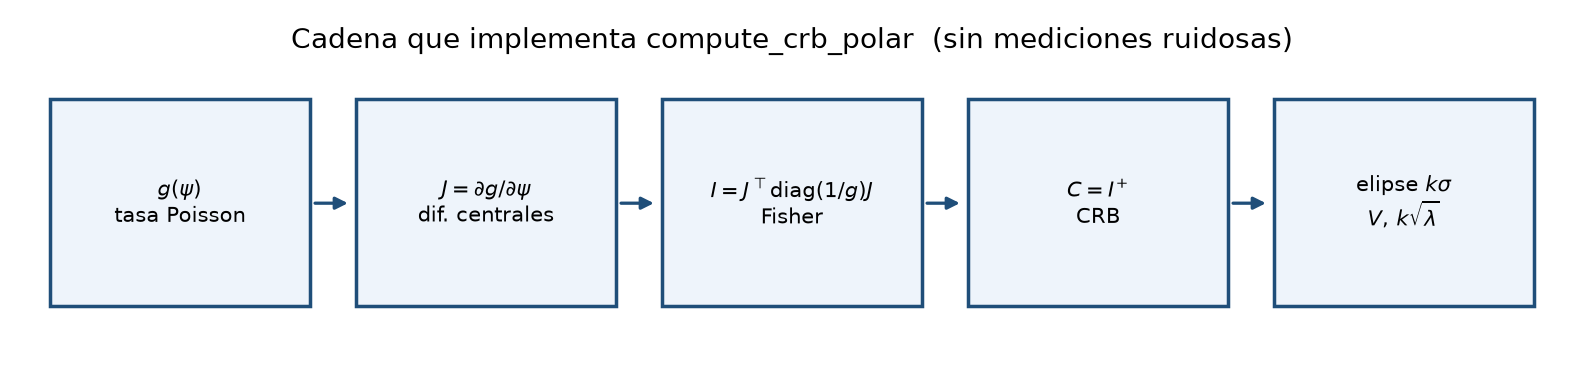
\includegraphics[width=0.98\textwidth]{pipeline.png}
\end{center}

%=======================================================================
\section{El objeto de partida: la tasa $g(\vect\psi)$}
\label{sec:g}

Sea $y(\vect\psi)$ el transitorio esperado que sale del simulador (sin ruido).
Cada \'indice $q$ enumera un par $(\text{p\'ixel},\,\text{\emph{bin}})$. Con
la grilla \emph{baseline} de $32\times32$ p\'ixeles y $95$ \emph{bins} hay
$N=97\,280$ \'indices. Se a\~nade un fondo constante
%
\begin{equation}
\label{eq:g}
g_q(\vect\psi) = y_q(\vect\psi) + b,
\qquad b = 0.1\ \text{cuentas/\emph{bin}},
\end{equation}
%
que en el c\'odigo es \code{forward\_g\_polar}:
\begin{center}\footnotesize
\code{background = background\_rate * ones\_like(y\_signal)}\\
\code{return y\_signal + background}
\end{center}
El valor $b=0.1$ es \code{BASELINE\_BACKGROUND\_RATE}.

Dos razones, una f\'isica y una matem\'atica:
%
\begin{itemize}[leftmargin=*]
  \item Un SPAD real tiene cuentas oscuras y luz ambiente; ning\'un \emph{bin}
        tiene tasa exactamente cero.
  \item Sin $b$, los miles de \emph{bins} vac\'ios tendr\'ian $g_q=0$ y el peso
        $1/g_q$ de la Fisher divergir\'ia. Con $b=0.1$ el piso num\'erico
        \code{fisher\_eps}$=10^{-12}$ de \code{fisher\_poisson} no llega a
        actuar.
\end{itemize}

El modelo de medici\'on, a partir de aqu\'i, es
%
\begin{equation}
\label{eq:poisson}
X_q \;\sim\; \mathrm{Poisson}\bigl(g_q(\vect\psi)\bigr)
\quad\text{independientes dado }\vect\psi.
\end{equation}
%
La propiedad que hace trabajar a todo lo que sigue es
%
\begin{equation}
\label{eq:var}
\operatorname{Var}(X_q)=\E[X_q]=g_q(\vect\psi).
\end{equation}
%
No hay un par\'ametro de ruido libre: el nivel de se\~nal fija la
incertidumbre. Por eso las constantes radiom\'etricas del \emph{forward}
(intensidad del l\'aser, fondo, n\'umero de p\'ixeles) \emph{s\'i} cambian el
CRB: no se cancelan al \enquote{normalizar}.

\begin{salvedad}[Independencia]
Distintos \emph{bins} temporales son ventanas disjuntas y distintos p\'ixeles
son detectores separados, as\'i que \eqref{eq:poisson} es razonable para un
contador ideal. Ignora tiempo muerto, diafon\'ia y \emph{jitter}. El CRB que
sale es por tanto el de un detector ideal: optimista frente a un sensor real.
\end{salvedad}

%=======================================================================
\section{Qu\'e significar\'ia estimar}
\label{sec:estimar}

Dada una realizaci\'on $\vect x$, la log-verosimilitud de Poisson es
%
\begin{equation}
\label{eq:loglik}
\ell(\vect\psi;\vect x)
= \sum_{q=1}^{N}
\bigl[\, x_q \ln g_q(\vect\psi) - g_q(\vect\psi) - \ln(x_q!)\,\bigr].
\end{equation}
%
El factorial no depende de $\vect\psi$. El estimador de m\'axima verosimilitud
(MV) ser\'ia
%
\begin{equation}
\label{eq:mle}
\hat{\vect\psi}_{\mathrm{MV}}(\vect x)
= \arg\max_{\vect\psi}\ell(\vect\psi;\vect x).
\end{equation}
%
Intuitivamente: se busca la pose cuya tasa esperada $g(\vect\psi)$ hace m\'as
probable el histograma observado. En un modelo regular, el MV es asint\'oticamente
insesgado, gaussiano y \textbf{alcanza} la CRB cuando $N$ es grande. Eso
justifica leer $\matr I^{-1}$ no solo como \enquote{nadie puede hacerlo mejor},
sino como \enquote{el MV, si se corriera, se parecer\'ia a esto}.

Tres precisiones evitan sobreinterpretarlo:
%
\begin{itemize}[leftmargin=*]
  \item Aqu\'i \textbf{no se corre} \eqref{eq:mle}. No hay garant\'ia num\'erica
        de que un optimizador sobre este \emph{forward} (que es escalonado)
        alcance la cota.
  \item La cota vale para estimadores \textbf{insesgados}. Un estimador sesgado
        puede tener varianza menor (el extremo, $\hat{\vect\psi}$ constante,
        tiene varianza cero) a costa del sesgo.
  \item Es \textbf{local}: $\matr I$ se eval\'ua en un $\vect\psi_0$ concreto y
        describe la curvatura de $\ell$ ah\'i. No detecta ambig\"uedades
        globales (dos poses lejanas con transitorios parecidos).
\end{itemize}

La \emph{score} ---el gradiente de $\ell$--- es lo que conecta estimar con
Fisher. Derivando \eqref{eq:loglik} respecto de la componente $m$,
%
\begin{equation}
\label{eq:score}
\frac{\partial\ell}{\partial\psi_m}
= \sum_q \frac{x_q - g_q}{g_q}\,
  \frac{\partial g_q}{\partial\psi_m}.
\end{equation}
%
Su esperanza es cero porque $\E[x_q]=g_q$: en media, la pendiente de $\ell$
en el valor verdadero es nula, que es la condici\'on de regularidad que usa
la CRB. La informaci\'on de Fisher es, por definici\'on, la covarianza de esa
pendiente:
%
\begin{equation}
\label{eq:def-fisher}
I_{mk}(\vect\psi)
= \E\Bigl[
    \frac{\partial\ell}{\partial\psi_m}\,
    \frac{\partial\ell}{\partial\psi_k}
  \Bigr].
\end{equation}
%
Un modelo \enquote{informativo} es uno cuya log-verosimilitud cambia de
pendiente de forma violenta cuando se mueve $\vect\psi$: la \emph{score} tiene
poca varianza alrededor de cero. Eso es exactamente lo que mide $\matr I$.

%=======================================================================
\section{De la \emph{score} a Fisher}
\label{sec:fisher}

Sustituyendo \eqref{eq:score} en \eqref{eq:def-fisher},
%
\begin{equation}
I_{mk}
= \sum_q\sum_{q'}
  \frac{\E[(x_q-g_q)(x_{q'}-g_{q'})]}{g_q\,g_{q'}}
  \frac{\partial g_q}{\partial\psi_m}
  \frac{\partial g_{q'}}{\partial\psi_k}.
\end{equation}
%
Aqu\'i entra la independencia. Si $q\neq q'$, $\E[(x_q-g_q)(x_{q'}-g_{q'})]=0$
y el t\'ermino cruzado desaparece. Si $q=q'$, la esperanza es la varianza, que
por \eqref{eq:var} vale $g_q$. Queda
%
\begin{equation}
\label{eq:fisher}
\boxed{\ 
I_{mk}(\vect\psi)
= \sum_{q=1}^{N}
  \frac{1}{g_q(\vect\psi)}
  \frac{\partial g_q}{\partial\psi_m}
  \frac{\partial g_q}{\partial\psi_k}\ }
\end{equation}
%
o, con el jacobiano $\matr J\in\mathbb R^{N\times 2}$,
$\matr J_{qm}=\partial g_q/\partial\psi_m$,
%
\begin{equation}
\label{eq:fisher-mat}
\matr I = \matr J^{\mathsf T}\,\diag(1/\vect g)\,\matr J.
\end{equation}
%
Esto es literalmente \code{fisher\_poisson}:
%
\begin{center}
\code{g\_safe = np.maximum(g, eps);  return J.T @ ((1.0/g\_safe)[:, None] * J)}.
\end{center}

\subsection{C\'omo leer cada t\'ermino}

La contribuci\'on del \'indice $q$ a $I_{mm}$ es
$(\partial g_q/\partial\psi_m)^2 / g_q$: sensibilidad al cuadrado sobre
varianza. Un \emph{bin} informa sobre $\rho$ si (i)~su tasa \emph{cambia} al
mover $\rho$ y (ii)~esa tasa no est\'a ahogada por su propio ruido de Poisson.
Los dos extremos aclaran la intuici\'on:
%
\begin{itemize}[leftmargin=*]
  \item se\~nal enorme pero insensible a la pose: numerador nulo, no aporta;
  \item muy sensible pero $g_q$ casi nulo: el denominador amplifica, y por eso
        los \emph{bins} del \emph{borde} del pulso (derivada alta, $g$ bajo)
        son los m\'as informativos.
\end{itemize}

El fondo $b$ \textbf{no a\~nade} informaci\'on. Los \'indices con
$\partial g_q/\partial\vect\psi=0$ contribuyen cero por muy grande que sea
$1/g_q$. Lo que hace $b$ es diluir los \emph{bins} que s\'i tienen se\~nal:
sube su varianza sin subir su sensibilidad. Subir $b$ empeora el CRB.

Dos propiedades estructurales:
%
\begin{itemize}[leftmargin=*]
  \item $\matr I$ es una \textbf{suma sobre mediciones}. M\'as p\'ixeles o
        m\'as \emph{bins} informativos a\~naden t\'erminos. Eso es lo que
        hace que, en \emph{este} modelo (que muestrea radiancia en el centro
        del p\'ixel, sin factor de \'area), $\sigma$ escale como $1/N$ al
        refinar una grilla $N\times N$.
  \item $\matr I$ es sim\'etrica y semidefinida positiva por construcci\'on
        ($\matr B^{\mathsf T}\matr B$ con
        $\matr B=\diag(1/\sqrt{\vect g})\matr J$). Sus autovalores son
        $\ge 0$ y la elipse de la secci\'on~\ref{sec:elipse} est\'a bien
        definida.
\end{itemize}

%=======================================================================
\section{El jacobiano: de $g$ a $J$ por diferencias finitas}
\label{sec:fd}

\eqref{eq:fisher} necesita $\partial g/\partial\vect\psi$. El \emph{forward}
contiene un $\lceil\cdot\rceil$ (asignaci\'on de \emph{bin}), un indicador de
oclusi\'on y cuatro $\max(0,\cdot)$ en los cosenos: no hay derivada cl\'asica
en todos los puntos. El \emph{pipeline} la aproxima por diferencias centrales,
%
\begin{equation}
\label{eq:fd}
\matr J_{:,m}
\approx
\frac{g(\vect\psi+\delta_m\vect e_m)-g(\vect\psi-\delta_m\vect e_m)}
     {2\,\delta_m},
\qquad
\vect\delta=(\delta_\rho,\delta_\varphi)=(0.01\,\mathrm{m},\,0.5^\circ),
\end{equation}
%
en \code{finite\_difference\_jacobian\_polar}. Cada pose cuesta $1+2\cdot 2=5$
evaluaciones: una central para $g(\vect\psi_0)$ y cuatro perturbadas.

\paragraph{Por qu\'e centrales.}
Si $g$ fuera suave,
$[g(\psi+\delta)-g(\psi-\delta)]/(2\delta)=g'(\psi)+O(\delta^2)$: los t\'erminos
pares se cancelan. Una diferencia unilateral ser\'ia $O(\delta)$. El
\emph{forward} es caro pero no prohibitivo; pagar una evaluaci\'on extra por
columna a cambio de un orden de precisi\'on es la elecci\'on correcta.

\paragraph{El problema honesto.}
$g$ \emph{no} es suave. Para un tri\'angulo aislado, mover $\rho$ en
$1\,\mathrm{cm}$ casi nunca cruza un borde de \emph{bin} ($c\Delta t\approx
11.7\,\mathrm{cm}$ de camino), y la derivada estimada sale $0$; cuando s\'i lo
cruza, salta una masa entera. Lo que rescata el c\'alculo es la suma sobre
$32\,768$ tri\'angulos: cada uno tiene su propio umbral, al mover $\rho$ una
fracci\'on proporcional a $\delta_\rho$ cruza, y el agregado se comporta como
una rampa. La suma sobre los $97\,280$ \'indices de \eqref{eq:fisher} cancela
adem\'as residuos de signo distinto. El resultado pr\'actico, medido en
$(1\,\mathrm{m},90^\circ)$, es que $\sigma_\varphi$ casi no se mueve al variar
$\delta_\rho$ en un factor $40$, y $\sigma_\rho$ crece de forma mon\'otona y
suave ($\sim 3\%$ entre el paso de $10\,\mathrm{mm}$ y el extrapolado a paso
cero). No demuestra diferenciabilidad; demuestra que el promediado basta para
que la cota no dependa de una elecci\'on arbitraria del paso.

El \emph{baseline} usa \code{float64} precisamente porque el numerador de
\eqref{eq:fd} resta dos n\'umeros parecidos. En \code{float32} esa cancelaci\'on
dejar\'ia pocos d\'igitos; elevados al cuadrado en $\matr I$ ser\'ian ruido.

%=======================================================================
\section{La cota: Fisher invertida es una covarianza}
\label{sec:crb}

\subsection{El enunciado}

Para cualquier estimador $\hat{\vect\psi}(\vect x)$ \textbf{insesgado} de
$\vect\psi$,
%
\begin{equation}
\label{eq:crb}
\Cov\bigl(\hat{\vect\psi}\bigr) \;\succeq\; \matr I(\vect\psi)^{-1},
\end{equation}
%
en el sentido de matrices: $\Cov-\matr I^{-1}$ es semidefinida positiva. En
particular, tomando diagonales,
$\operatorname{Var}(\hat\rho)\ge [\matr I^{-1}]_{11}$ y
$\operatorname{Var}(\hat\varphi)\ge [\matr I^{-1}]_{22}$. El c\'odigo define
%
\begin{equation}
\label{eq:C}
\matr C = \matr I^{+},
\qquad
\sigma_\rho=\sqrt{C_{11}},
\qquad
\sigma_\varphi=\sqrt{C_{22}},
\qquad
\sigma_{\mathrm{tang}}=\rho\,\sigma_\varphi,
\end{equation}
%
en \code{\_crb\_sigmas\_from\_matrix}. $\sigma_{\mathrm{tang}}$ pasa
$\sigma_\varphi$ (radianes) a metros de arco en la pose nominal, para
compararlo con $\sigma_\rho$ en las mismas unidades.

Se usa \code{np.linalg.pinv} y no \code{inv}. Si en alguna pose una direcci\'on
de $\vect\psi$ no fuera observable, $\matr I$ ser\'ia singular e \code{inv}
abortar\'ia la rejilla. La pseudoinversa anula esa direcci\'on y deja que las
$\sigma$ delaten el problema. En las $15$ poses del \emph{baseline} $\matr I$
est\'a bien condicionada y ambas coinciden.

\subsection{Qu\'e es y qu\'e no es $\matr C$}

$\matr C$ es la \textbf{covarianza m\'inima} de $(\hat\rho,\hat\varphi)$, no un
histograma de errores medidos. Sus unidades son
%
\[
C_{11}\ \text{en m}^2,\quad
C_{22}\ \text{en rad}^2,\quad
C_{12}\ \text{en m}\cdot\text{rad}.
\]
%
Los $\sigma$ de \eqref{eq:C} son las incertidumbres \textbf{conjuntas}: las de
estimar $\rho$ y $\varphi$ \emph{a la vez}. La incertidumbre condicional (si
$\varphi$ se conociera de antemano) ser\'ia $1/\sqrt{I_{\rho\rho}}$, siempre
menor o igual:
%
\begin{equation}
\label{eq:cond}
\sigma_\rho
= \frac{1}{\sqrt{I_{\rho\rho}}}\cdot\frac{1}{\sqrt{1-r_I^2}},
\qquad
r_I=\frac{I_{\rho\varphi}}{\sqrt{I_{\rho\rho}I_{\varphi\varphi}}}.
\end{equation}
%
Estimar un par\'ametro extra nunca sale gratis: la correlaci\'on infla las
$\sigma$ marginales. Ese es el mismo mecanismo por el que, cuando el CRB ten\'ia
tres par\'ametros $(\rho,\varphi,h)$, a\~nadir la altura ensanchaba las
burbujas en $(\rho,\varphi)$.

\subsection{La correlaci\'on}

El t\'ermino fuera de la diagonal se reporta como
%
\begin{equation}
\label{eq:corr}
r_{\rho\varphi}
= \frac{C_{12}}{\sqrt{C_{11}C_{22}}}.
\end{equation}
%
$I_{\rho\varphi}=\sum_q g_q^{-1}(\partial_\rho g_q)(\partial_\varphi g_q)$ se
anular\'ia solo si ninguna medici\'on fuera sensible a ambos par\'ametros a la
vez. Aqu\'i ocurre lo contrario: el camino $d_1+d_2$ depende de
$(\rho\cos\varphi,\rho\sin\varphi)$, y la frontera de oclusi\'on tambi\'en.
Mover $\rho$ desplaza la sombra, que es precisamente el mecanismo que informa
sobre $\varphi$.

En toda la rejilla \emph{baseline} $r_{\rho\varphi}<0$: una sobreestimaci\'on de
$\rho$ tiende a ir con una subestimaci\'on de $\varphi$. Existe una
\textbf{direcci\'on de compensaci\'on} a lo largo de la cual el transitorio
cambia poco (alejar la faceta y girarla hacia el hueco produce, al primer
orden, un camino y una sombra parecidos). El estimador distingue bien el
desplazamiento perpendicular a esa direcci\'on y mal el paralelo. Eso es la
elipse alargada e inclinada.

\begin{obs}[Coordenadas independientes, estimadores correlacionados]
$\rho$ y $\varphi$ se pueden fijar por separado: nada las liga \emph{a priori}.
Lo correlacionado son los \textbf{errores de sus estimaciones}, porque los
datos no las separan limpiamente. Son afirmaciones sobre objetos distintos.
\end{obs}

%=======================================================================
\section{De la matriz a la elipse}
\label{sec:elipse}

\subsection{La regi\'on de Mahalanobis}

Una covarianza $2\times 2$ definida positiva define una familia de elipses.
Para un error $\vect\delta=\vect\psi-\vect\psi_0$,
%
\begin{equation}
\label{eq:region}
\mathcal E_k
= \bigl\{\,
    \vect\delta\in\mathbb R^2 :
    \vect\delta^{\mathsf T}\matr C^{-1}\vect\delta \le k^2
  \,\bigr\}
\end{equation}
%
es el conjunto de desplazamientos cuya distancia de Mahalanobis a $\vect\psi_0$
es a lo sumo $k$. La forma cuadr\'atica $\vect\delta^{\mathsf T}\matr C^{-1}
\vect\delta$ vale $1$ sobre la elipse de covarianza \enquote{unidad} y $k^2$
sobre la de radio $k$: \textbf{el n\'umero $k$ no cambia la forma, solo la
escala}.

Como $\matr C$ es sim\'etrica definida positiva existe
%
\begin{equation}
\label{eq:eig}
\matr C = \matr V\matr\Lambda\matr V^{\mathsf T},
\qquad
\matr\Lambda=\diag(\lambda_1,\lambda_2),\quad
\matr V\text{ ortogonal}.
\end{equation}
%
El cambio $\vect\delta = \matr V\matr\Lambda^{1/2}\vect u$ convierte
\eqref{eq:region} en $\|\vect u\|\le k$. La frontera es por tanto la imagen
de un c\'irculo de radio $k$:
%
\begin{equation}
\label{eq:ellipse}
\vect\delta(\vartheta)
= k\,\matr V\matr\Lambda^{1/2}
  \begin{pmatrix}\cos\vartheta\\ \sin\vartheta\end{pmatrix},
\qquad \vartheta\in[0,2\pi).
\end{equation}
%
Semiejes $k\sqrt{\lambda_i}$, orientados seg\'un los autovectores de $\matr C$.
Eso es exactamente la funci\'on
\code{crb\_region\_in\_polar\_parameters}:
%
\begin{center}
\footnotesize
\code{evals, evecs = np.linalg.eigh(Sigma)}\\
\code{axes = k * np.sqrt(evals)}\\
\code{ellipse = center[:,None] + evecs @ np.diag(axes) @ circle}
\end{center}
%
con el c\'irculo unidad muestreado en $300$ puntos y
\code{np.maximum(eigenvalues, 0)} como guarda contra autovalores
ligeramente negativos por redondeo. El bloque $\Sigma$ es
$\matr C[\{0,1\},\{0,1\}]$; con Fisher $2\times 2$ es $\matr C$ entero.

\begin{figure}[htbp]
\centering
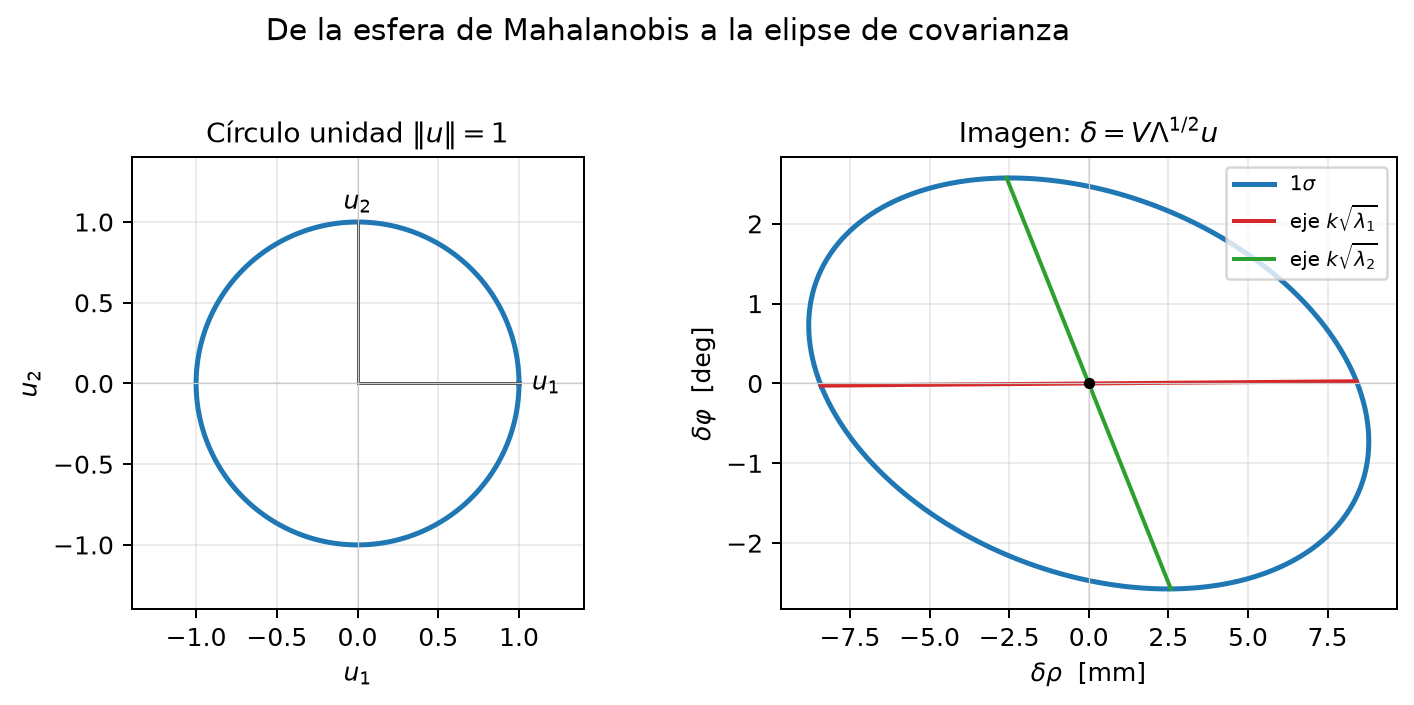
\includegraphics[width=0.98\textwidth]{mahalanobis.png}
\caption{Izquierda: el c\'irculo $\|\vect u\|=1$ en las coordenadas
blanqueadas. Derecha: su imagen bajo $\matr V\matr\Lambda^{1/2}$, que es la
elipse $1\sigma$ en $(\delta\rho,\delta\varphi)$. Los ejes de color son
$k\sqrt{\lambda_i}$ con $k=1$. Pose $(1\,\mathrm{m},90^\circ)$, CRB
\emph{baseline} $32\times 32$.}
\label{fig:mahal}
\end{figure}

\subsection{Por qu\'e $k=3$ (y qu\'e cambia $k=1$)}

Si los errores fueran gaussianos de covarianza $\matr C$, la forma cuadr\'atica
$\vect\delta^{\mathsf T}\matr C^{-1}\vect\delta$ seguir\'ia una $\chi^2$ con
$2$ grados de libertad, cuya funci\'on de distribuci\'on es
$F(u)=1-e^{-u/2}$. Entonces
%
\begin{equation}
\label{eq:cobertura}
\Pr(\vect\delta\in\mathcal E_k) = 1-e^{-k^2/2}.
\end{equation}

\begin{center}
\begin{tabular}{@{}cccc@{}}
\toprule
$k$ & cobertura 2D \eqref{eq:cobertura} & tama\~no lineal vs $1\sigma$ & \'area vs $1\sigma$ \\
\midrule
$1$ & $1-e^{-1/2}=39.3\%$ & $1$ & $1$ \\
$2$ & $1-e^{-2}=86.5\%$ & $2$ & $4$ \\
$3$ & $1-e^{-4.5}=98.9\%$ & $3$ & $9$ \\
\bottomrule
\end{tabular}
\end{center}

El \emph{pipeline} usa $k=3$ por defecto (\code{k=3.0} en
\code{compute\_crb\_polar}). Es una regi\'on de \textbf{casi-cobertura}: si el
error fuera gaussiano, el valor verdadero cae dentro en el $98.9\%$ de las
realizaciones. No es la regla unidimensional de \enquote{$\pm 3\sigma$ cubre
el $99.73\%$}: en 2D hay m\'as sitio fuera, y la misma $k$ cubre solo el
$98.9\%$.

$k=1$ es la elipse de \textbf{error t\'ipico}: semiejes $\sigma$ a lo largo de
las direcciones principales. Sirve para leer a ojo \enquote{cu\'anto se suele
fallar}. $k=3$ responde a otra pregunta ---\enquote{d\'onde cae casi seguro}---
y por construcci\'on se ve tres veces m\'as ancha y nueve veces m\'as grande
en \'area. \textbf{No cambia la CRB}; cambia el zoom de la curva.

\begin{figure}[htbp]
\centering
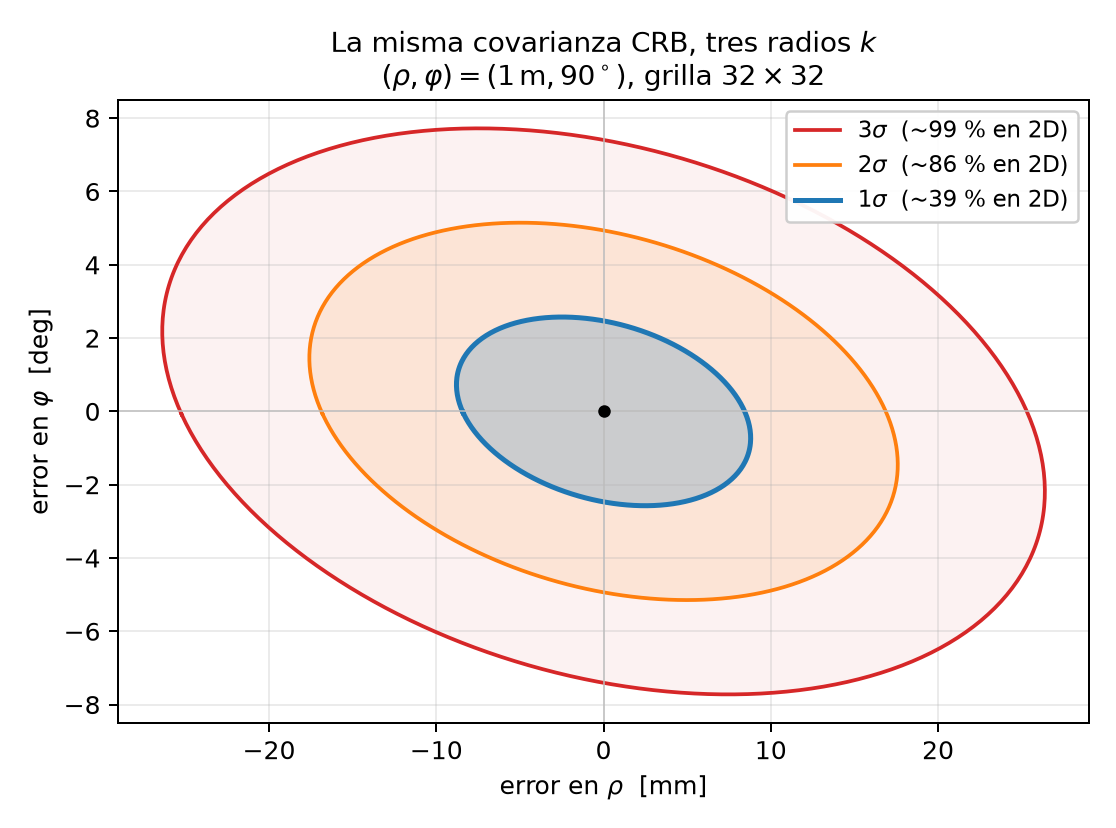
\includegraphics[width=0.78\textwidth]{sigma_scales.png}
\caption{Las tres escalas sobre la misma matriz $\matr C$ de
$(1\,\mathrm{m},90^\circ)$. La inclinaci\'on es $r_{\rho\varphi}=-0.28$; el
alargamiento es $\sigma_{\mathrm{tang}}/\sigma_\rho\approx 5$. Pasar de $1\sigma$
a $3\sigma$ no \enquote{empeora} la cota: multiplica los semiejes por $3$.}
\label{fig:escalas}
\end{figure}

\subsection{La inclinaci\'on \emph{es} la correlaci\'on}

Si $r_{\rho\varphi}=0$, $\matr C$ es diagonal, los autovectores son los ejes
coordenados y la elipse sale alineada con $(\rho,\varphi)$. Si
$r_{\rho\varphi}\neq 0$, giran un \'angulo $\alpha$ que cumple
%
\begin{equation}
\label{eq:tilt}
\tan(2\alpha)=\frac{2C_{12}}{C_{11}-C_{22}}.
\end{equation}
%
Con $C_{12}<0$ en toda la rejilla, el eje mayor apunta hacia
\enquote{$\rho$ arriba, $\varphi$ abajo}: mirar la inclinaci\'on de una
burbuja es leer la direcci\'on de compensaci\'on de la
secci\'on~\ref{sec:crb}.

Los autovalores mismos mezclan metros y radianes, as\'i que el \enquote{\'angulo
de inclinaci\'on} y la relaci\'on de semiejes dependen de la unidad en que se
mida $\varphi$. No es un error: es una convenci\'on. Mientras se aplique la
misma a todas las poses, las comparaciones son v\'alidas. Lo invariante son
$\sigma_\rho$, $\sigma_\varphi$ por separado, y $\rho\,\sigma_\varphi$ en
metros.

%=======================================================================
\section{C\'omo se dibuja (y por qu\'e se ve arqueada)}
\label{sec:dibujo}

Hay dos representaciones de $\mathcal E_k$. El \emph{pipeline} usa la primera.

\paragraph{Burbujas en el plano de par\'ametros.}
Se toma \eqref{eq:ellipse} centrada en $(\rho_0,\varphi_0)$ y se pinta sobre
ejes polares con \code{ax.plot(phi\_curve, rho\_curve)}: $\varphi$ como
\'angulo, $\rho$ como radio. Es
\code{plot\_crb\_regions\_polar} con
\code{use\_physical\_region=False}. Se elige esta v\'ia porque \textbf{el CRB vive
en el espacio de par\'ametros}: sus semiejes \emph{son} $\sigma_\rho$ y
$\sigma_\varphi$ (mezclados por la correlaci\'on). No hay transformaci\'on
intermedia.

\paragraph{Gotas en el plano f\'isico $xy$.}
La alternativa, implementada en \code{crb\_region\_physical\_xy\_to\_polar}
y apagada por defecto, transporta $\matr C$ con la linealizaci\'on
%
\begin{equation}
\label{eq:push}
\matr A
= \frac{\partial(x,y)}{\partial(\rho,\varphi)}
= \begin{pmatrix}
    \cos\varphi & -\rho\sin\varphi \\
    \sin\varphi & \rho\cos\varphi
  \end{pmatrix},
\qquad
\Sigma_{xy}=\matr A\,\matr C\,\matr A^{\mathsf T}.
\end{equation}
%
Es una aproximaci\'on de primer orden: la imagen exacta de una elipse por el
mapa polar$\to$cartesiano \emph{no} es una elipse, y al reconvertir a polares
para el dibujo el contorno se curva en forma de gota. Esa asimetr\'ia no est\'a
en la CRB; est\'a en el cambio de coordenadas. Por eso se abandon\'o.

\begin{figure}[htbp]
\centering
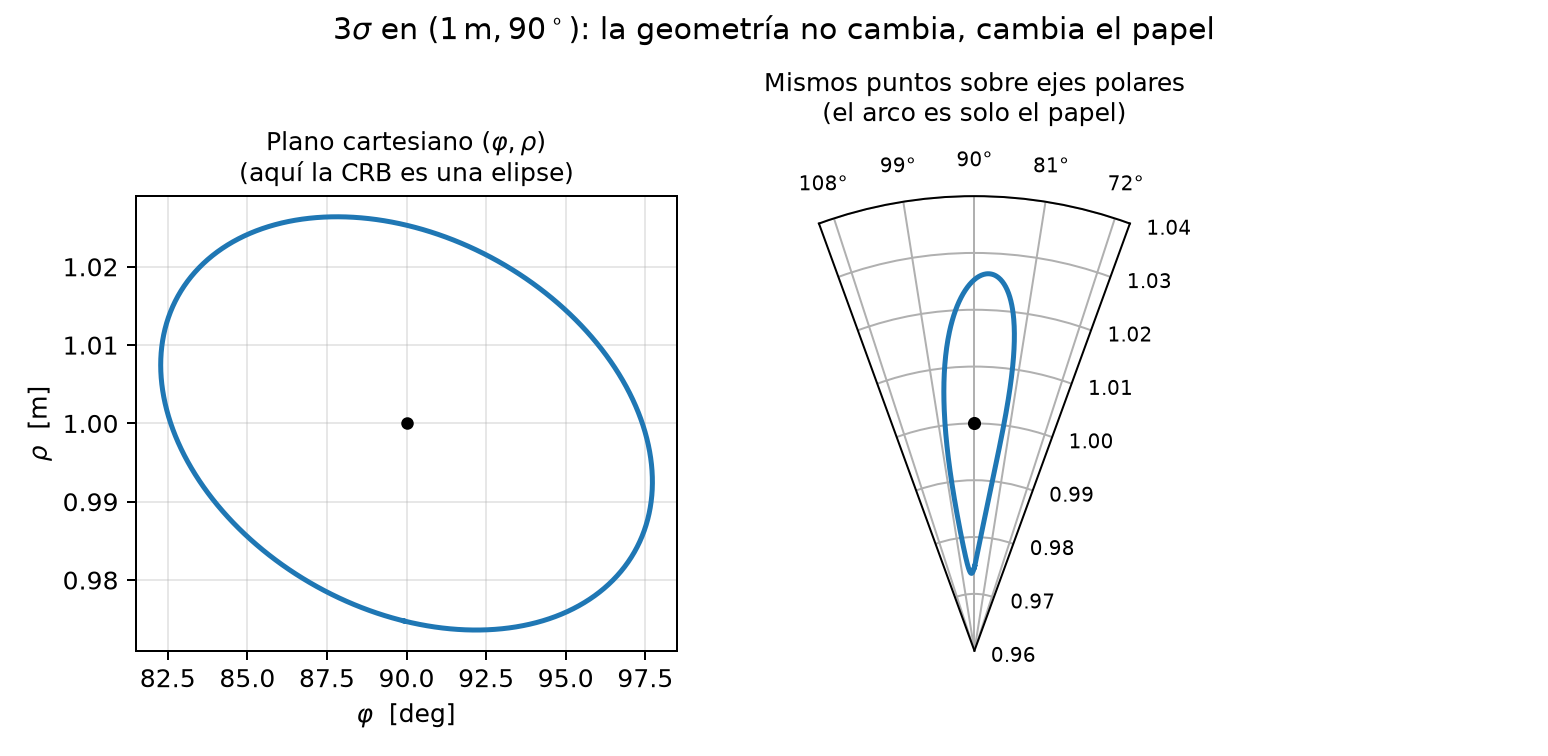
\includegraphics[width=0.98\textwidth]{polar_warp.png}
\caption{La misma elipse $3\sigma$ de $(1\,\mathrm{m},90^\circ)$. Izquierda:
plano cartesiano $(\varphi,\rho)$, donde \eqref{eq:ellipse} es una elipse
eucl\'idea. Derecha: los mismos puntos sobre ejes polares; un segmento de
$\rho$ constante se vuelve un arco, y la curva se ve \enquote{arqueada}. No es
una deformaci\'on de la cota.}
\label{fig:polar}
\end{figure}

El estilo polar (\code{\_style\_polar\_crb\_ax}) fija medio plano
$\theta\in[0^\circ,180^\circ]$, cero a la derecha, sentido antihorario,
etiquetas radiales a dos decimales. Con \code{rlim=2.0} las quince poses
$\rho\in\{0.5,1.0,1.5\}\,\mathrm{m}$ caben en el mismo marco. Eso tiene un
coste de lectura: a $3\sigma$ y $\rho=1.5\,\mathrm{m}$, $\sigma_\varphi$ de
varios grados produce arcos que ocupan un sector enorme, mientras las de
$\rho=0.5\,\mathrm{m}$ quedan como puntos. No es que la CRB de cerca sea
nula; es que comparte escala con la de lejos.

\begin{figure}[htbp]
\centering
\IfFileExists{../plots/crb_fd_baseline_32.png}{%
  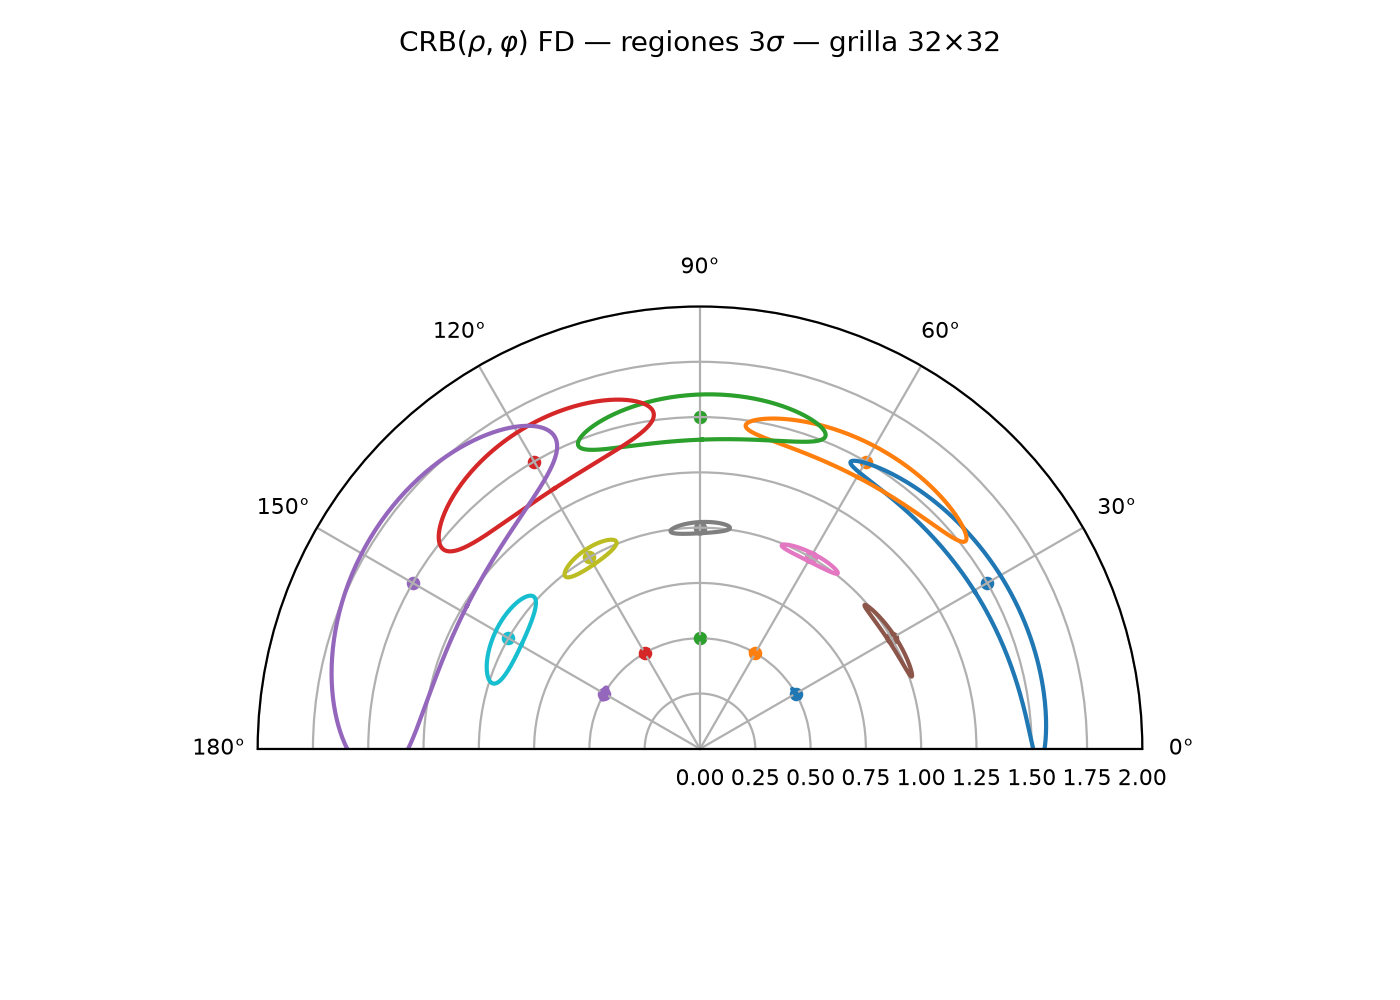
\includegraphics[width=0.72\textwidth]{crb_fd_baseline_32.png}}{%
  \fbox{\parbox{0.85\textwidth}{\centering\vspace{1.5em}(figura
  \code{plots/crb\_fd\_baseline\_32.png} no disponible)\vspace{1.5em}}}}
\caption{Salida de \code{compute\_crb\_fd\_baseline.py}: regiones $3\sigma$ en
el plano $(\rho,\varphi)$, grilla $32\times 32$. Cada burbuja es
\eqref{eq:ellipse} con $k=3$, centrada en su pose. El aspecto \enquote{horrible}
de las de $\rho=1.5\,\mathrm{m}$ es $3\sigma_\varphi$ de $22^\circ$--$35^\circ$
dibujado como arco polar, no un fallo del trazo.}
\label{fig:baseline}
\end{figure}

%=======================================================================
\section{C\'omo leer una burbuja}
\label{sec:leer}

Una elipse del gr\'afico resume cuatro n\'umeros, no uno.
%
\begin{enumerate}[leftmargin=*]
  \item \textbf{Anchura radial} $\approx 2k\sigma_\rho$: cu\'anto se puede
        fallar en rango. El tiempo de vuelo mide $\rho$ de forma bastante
        directa, as\'i que este semieje suele ser el corto.
  \item \textbf{Anchura angular} $\approx 2k\sigma_\varphi$: cu\'anto se puede
        fallar en azimut. $\varphi$ se infiere de la geometr\'ia de la sombra;
        $\rho\,\sigma_\varphi$ es varias veces $\sigma_\rho$ y el eje mayor
        es casi tangencial.
  \item \textbf{Inclinaci\'on}: signo y magnitud de $r_{\rho\varphi}$. Todas
        las del \emph{baseline} se inclinan en el mismo sentido porque todas
        las correlaciones son negativas.
  \item \textbf{Radio $k$}: si es $3$, se est\'a viendo casi-cobertura
        ($\sim 99\%$ gaussiano 2D), no el error t\'ipico. Para comparar
        m\'etodos a ojo, $k=1$ es m\'as honesto; para citar una regi\'on de
        confianza, $k=3$ es el que usa el c\'odigo.
\end{enumerate}

Nada de eso es el error de un estimador que se haya corrido. Es la cota: el
suelo de la covarianza de cualquier estimador insesgado de $(\rho,\varphi)$
bajo el modelo de Poisson \eqref{eq:poisson} y el \emph{forward} $g$ que se
haya usado para construir $\matr J$.

%=======================================================================
\section{Mapa al c\'odigo}
\label{sec:mapa}

{\footnotesize
\begin{center}
\begin{tabular}{@{}p{6.6cm}p{8.2cm}@{}}
\toprule
Funci\'on en \code{crb\_polar\_functions.py} & Paso de este texto \\
\midrule
\code{forward\_g\_polar} &
  $g=y+b$, ecuaci\'on~\eqref{eq:g} \\
\code{finite\_difference\_jacobian\_polar} &
  $J$, ecuaci\'on~\eqref{eq:fd} \\
\code{fisher\_poisson} &
  $I=J^{\mathsf T}\diag(1/g)J$, ecuaci\'on~\eqref{eq:fisher-mat} \\
\code{np.linalg.pinv} (en \code{compute\_crb\_polar}) &
  $C=I^{+}$, ecuaci\'on~\eqref{eq:C} \\
\code{\_crb\_sigmas\_from\_matrix} &
  $\sigma_\rho$, $\sigma_\varphi$, $\rho\sigma_\varphi$ \\
correlaci\'on en \code{compute\_crb\_polar} &
  $r_{\rho\varphi}$, ecuaci\'on~\eqref{eq:corr} \\
\code{crb\_region\_in\_polar\_parameters} &
  elipse \eqref{eq:ellipse} en $(\rho,\varphi)$ \\
\code{crb\_region\_physical\_xy\_to\_polar} &
  empuje a $xy$ \eqref{eq:push} (no se dibuja) \\
\code{plot\_crb\_regions\_polar} &
  burbujas; \code{use\_physical\_region=False} \\
\bottomrule
\end{tabular}
\end{center}
}

El \emph{script} \code{compute\_crb\_fd\_baseline.py} recorre las $15$ poses
$(\rho,\varphi)$ con \code{estimate\_height=False}, $k=3$ y \code{rlim=2.0},
y escribe \code{plots/crb\_fd\_baseline\_32.png}. Las figuras de este
documento se regeneran con
\begin{center}
\code{python3 docs/figs\_crb\_ellipses/make\_figs.py}
\end{center}

\end{document}
